\documentclass[a4paper,12pt]{article}
\usepackage{graphicx}
\begin{document}

\centerline{\huge \textbf{Testing documentation}} \hspace*{\fill}
\\
Most of the code's classes have a set of \emph{unit tests} that are run automatically after compiling. GUI and geometry tools are not tested. Following are the descriptions of all implemented automatic tests, all of which pass everytime.\\

\paragraph{\large VertexContainer} \hspace{0pt} \\
Tests if Vertex and Point are added at coordinates (3,5)\\
Tests if Vertex and Point can be removed.\\
Checks if an \emph{edge} between two vertices can be toggled. \emph{toggleEdge} is called two times, after first call edge should exist but after second call it shouldn't. Another test calls \emph{toggleEdge} 1000 times.\\
Another test calls \emph{buildGraph}, simultaneously testing AngleElimination algorithm. Test places points at static positions, calls \emph{buildGraph} and checks if the graph is correct. Visualisation of the test:\\
\centerline{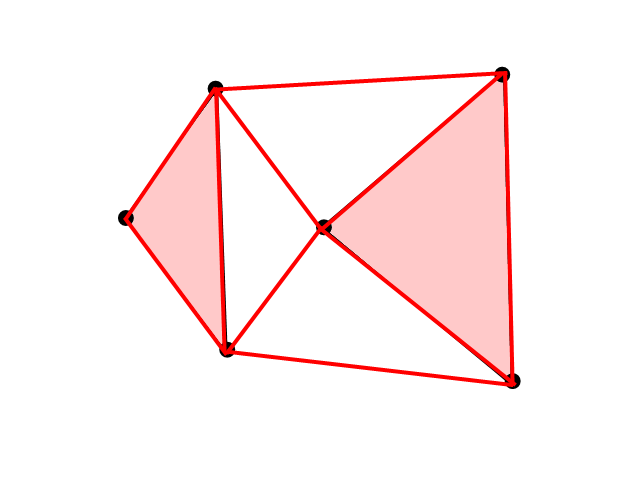
\includegraphics[scale=0.25]{vc.png}} \hspace*{\fill} \\
Places three points on a triangle clockwise, which should form a wall polygon. Also places three points counter clockwise, which should form a non-wall polygon.\\
Another test places points to form a non-wall triangle and then calls\\ \emph{invertShape}, after which triangle should be a wall.\\

\paragraph{\large AngleElimination} \hspace{0pt} \\
Places a vertex \emph{v} and several triangles in a specific way, after which\\ AngleElimination is called from the point of view of \emph{v}. Test checks if algorithm returned a correct set of \emph{unobstructed} points. Visualisation of the test, where \emph{v} is colored green and unobsturcted points are colored blue:\\
\centerline{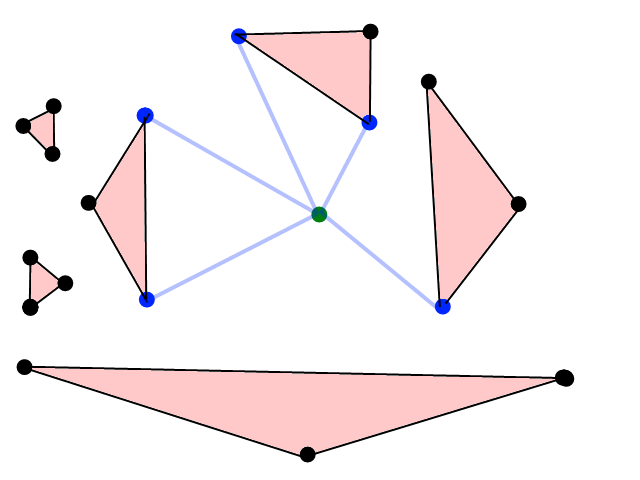
\includegraphics[scale=0.5]{ae.png}} \hspace*{\fill} \\

\paragraph{\large Dijkstra} \hspace{0pt} \\
Three different graphs are built with end points, after which test checks if Dijkstra's returned path is the shortest one. Visualisations of the test, where starting vertex is colored red, ending vertex blue, and shortest path is colored green:\\
\centerline{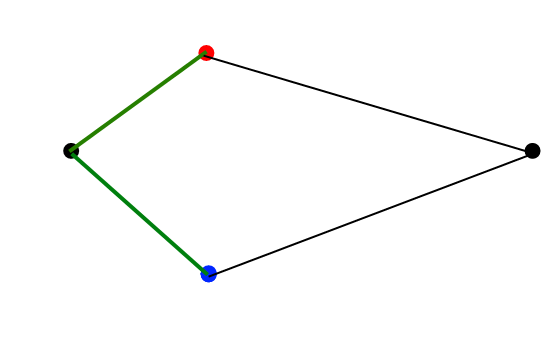
\includegraphics[scale=0.5]{dij1.png}} \hspace*{\fill} \\
\centerline{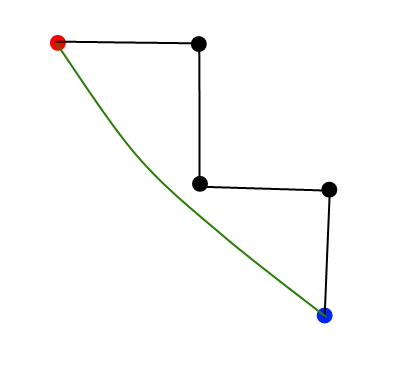
\includegraphics[scale=0.5]{dij2.png}} \hspace*{\fill} \\
\centerline{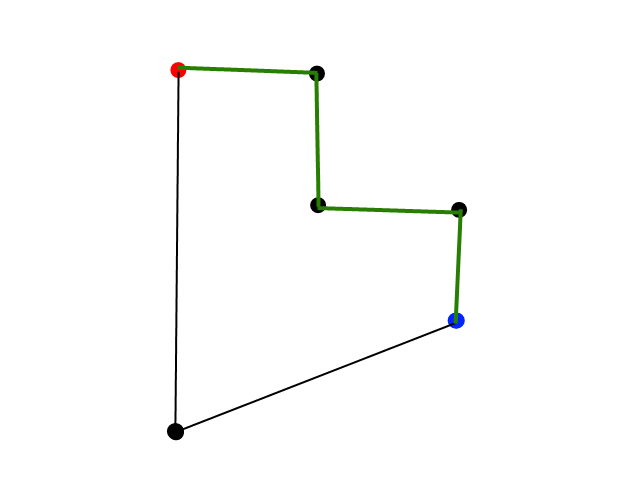
\includegraphics[scale=0.5]{dij3.png}} \hspace*{\fill} \\

\paragraph{\large Heap} \hspace{0pt} \\
Checks if Heap always \emph{pops} the smallest element. 1000 random integers are \emph{inserted} into the heap, after which heap is popped until it's \emph{empty}. Test passes if next popped integer is never smaller than previously popped integer.\\
Checks if Heap is empty when \emph{clear} is called. Before calling \emph{clear} Heap is filled with random integers.\\
1337 random integers are added to the Heap, after which \emph{size} is called, which should return 1337.\\
Checks if calling \emph{pop} will reduce Heap's \emph{size} by one.\\
Heap's original array size is 15. Test inserts 14 elements, after which array size shouldn't change. After inserting one more element, array size should be doubled.\\
Following integers are inserted in following order: 1, 3, 5, 7, 9, 11, 13, 15, 17, 19, 21, 23, 25, 27, 29, 6. Heap's array should now be in the following order: 1, 3, 5, 6, 9, 11, 13, 7, 17, 19, 21, 23, 25, 27, 29, 15.\\
Integers from 1-15 are inserted to the Heap in ascending order. Heap is popped, after which Heap's array should be in the following order: 2, 4, 3, 8, 5, 6, 7, 15, 9, 10, 11, 12, 13, 14.\\
Following integers are inserted in following order: 1, 3, 5, 7, 9, 11, 13, 15, 17, 19, 21, 23, 25, 27, 29. Then, 19's value is changed to 2. Heap's array should now be in the following order: 1, 2, 5, 7, 3, 11, 13, 15, 17, 9, 21, 23, 25, 27, 29.\\
Following integers are inserted in following order: 1, 3, 5, 7, 9, 11, 13, 15, 17, 19, 21, 23, 25, 27, 29. Then, 5's value is changed to 26. Heap's array should now be in the following order: 1, 3, 11, 7, 9, 23, 13, 15, 17, 19, 21, 26, 25, 27, 29.\\
\\
\emph{Note about changing values of existing integers: Integers had to be reimplemented in order to have two identifiable attributes. One is its value, which is what is tested and represented in this document. Other is its ID, which can never be changed. This is needed in order to find the correct integer from the TreeMap with indexes.}\\
\\
1337 integers are added to the heap, one of them is 1, which is the smallest integer in the Heap. \emph{peek} is called 1337 times. Returned value should be 1 every time, and Heap's size shouldn't change.\\
TreeMap's contents are checked. For every added element \emph{e}, TreeMap should return an index \emph{i}, where \emph{array[i] = e}. \emph{Note: test works correctly if all integers in the Heap are unique.}

\paragraph{\large LinkedList} \hspace{0pt} \\
Several elements are \emph{added} and then \emph{iterated}. Test checks if correct elements are returned in correct order. Also, after all elements are iterated, \emph{getNext} should return null.\\
1337 elements are added, after which \emph{size} should return 1337.\\
1337 elements are added and \emph{clear} is called. \emph{isEmpty} should return true.\\
\emph{clear} is called, after which \emph{getNext} should return null.\\
1337 elements are added, \emph{clear} is called and 13 elements are added after that. Now \emph{size} should return 13.\\
1337 elements are added and \emph{getNext} is called 1337 times. \emph{getNext} should never return null.\\
1337 elements are added and \emph{hasNext} is called 1337 times paired with\\ \emph{getNext}. It should never be false, except if called for the 1338'th time.\\
4 elements are added and iterated. After calling \emph{reset}, LinkedList should be able to be iterated another time.\\
1338 elements are added and \emph{getNext} is called 478 times. After calling \emph{reset}, \emph{getNext} should return the first element.

\paragraph{\large Point} \hspace{0pt} \\
Point is placed at (0,0). Left and right neighbours are then placed at several locations, while forming a $180^{\circ}$ angle. Point's angle should return $180^{\circ}$ every time.\\
Point is placed, whose angle is less than $180^{\circ}$ and another with more than $180^{\circ}$ angle. First point should return false for \emph{isVertex}, while other should return true.

\paragraph{\large Queue} \hspace{0pt} \\
For every test, four elements are \emph{enqueued}.\\
\emph{dequeue} is called five times. Each time \emph{dequeue} should return a correct value, the fifth time should return null.\\
\emph{dequeue} is called three times, after which new element is \emph{enqueued}. Now \emph{dequeue} should return the fourth element, and next \emph{dequeue} should return the newly added element. After that \emph{dequeue} should return null.\\
After calling \emph{clear isEmpty} should return true.\\
\emph{clear} is called and a new element is enqueued.  Now \emph{dequeue} should return the new element. Another \emph{dequeue} returns null.\\
Queue is cleared and elements are queued a random \emph{r} amount of times. Then elements are dequeued a random \emph{b} amount of times, where b \textless{ r}. \emph{size} should return \emph{r - b}. This test is then repeated 10000 times.

\paragraph{\large TreeMap} \hspace{0pt} \\
Three key-value pairs are \emph{put} into the TreeMap for every test.\\
Calling \emph{get} for every \emph{key} returns a appropriate \emph{value}.\\
If \emph{put} is called for existing key, that key should return the new value.\\
If \emph{get} is called for a key that doesn't exist in the TreeMap, null should be returned.

\paragraph{\large Tree} \hspace{0pt} \\
1024 integers are \emph{added} in ascending order. Tree's height should be less than 20.\\
1024 integers are added in descending order. Tree's height should be less than 20.\\
1024 integers are added in random order. Tree's height should be less than 20.\\
2048 integers are added in ascending order and 1024 first integers are\\ \emph{removed}. Tree's height should be less than 20.\\
2048 integers are added in random order and 1024 random integers are removed. Tree's height should be less than 20.\\
2048 integers are added and \emph{clear} is called. \emph{isEmpty} should return true.\\
2048 integers are added in ascending order and \emph{toLinkedList} is called. Returned LinkedList should contain all integers from 1 to 2048.\\
Integer 0 is added among with 2048 random integers, which are bigger than 0. \emph{getMin} should return 0.\\
Tree is cleared. Now \emph{getMin} should return null.\\
Tree is cleared and integers are added in ascending order a random \emph{r} amount of times. Then elements are removed in ascending order a random \emph{b} amount of times, where b \textless{ r}. \emph{size} should return \emph{r - b}. This test is then repeated 10000 times.\\
Tree is cleared. 1000 integers are added in ascending order. Tree should now contain an integer, value of which is between 1 and 1000. This test is then repeated 1000 times.\\
Integers from 1 to 1000 are added. \emph{contains(-1)} should return false.

\paragraph{\large Vertex} \hspace{0pt} \\
Two vertices are placed. One vertex is \emph{added} for the other as \emph{adjacent}. Now vertices should have each other in their \emph{adjacent tree}.\\
One vertex is placed and the same vertex is added as adjacent. Adjacent tree should be empty.\\
Two vertices are placed. One vertex is added for the other as adjacent. Then, one vertex is removed from other's adjacent tree. Now both adjacent trees should be empty.\\
A vertex is placed. 1000 vertices are added to the vertex as adjacents. After calling \emph{removeAllAdjacents}, adjacent tree must be empty.\\
One vertex is placed at (0,0), other is placed at (3,4). When measuring distance from either vertex to the other, distance should be 5.\\
One vertex \emph{$v_1$} is placed at (0,0), other \emph{$v_2$} is placed at (1,1). Direction from \emph{$v_1$} to \emph{$v_2$} must be $45^{\circ}$, and $-135^{\circ}$ vice versa.\\
\emph{src} is placed at (0,0), \emph{v} is placed at (1,0), \emph{left} at (1,-1) and \emph{right} at (1,1). Now, \emph{src} should recognise that \emph{v} is between \emph{left} and \emph{right}.\\
\emph{src} is placed at (0,0), \emph{v} is placed at (-1,0), \emph{left} at (-1,1) and \emph{right} at (-1,-1). Now, \emph{src} should recognise that \emph{v} is between \emph{left} and \emph{right}.\\
\emph{src} is placed at (0,0), \emph{v} is placed at (-1,0), \emph{left} at (1,-1) and \emph{right} at (1,1). Now, \emph{src} should recognise that \emph{v} \textbf{isn't} between \emph{left} and \emph{right}.\\
\emph{src} is placed at (0,0), \emph{v} is placed at (1,0), \emph{left} at (-1,1) and \emph{right} at (-1,-1). Now, \emph{src} should recognise that \emph{v} isn't between \emph{left} and \emph{right}.\\

\paragraph{\large Tools} \hspace{0pt} \\
\emph{round} is tested with several parameters. Specific parameters should be evident from test's code.\\
$0^{\circ}$ should be between $-45^{\circ}$ and $45^{\circ}$\\
$180^{\circ}$ should be between $135^{\circ}$ and $-135^{\circ}$\\
$-180^{\circ}$ shouldn't be between $-45^{\circ}$ and $45^{\circ}$\\
$0^{\circ}$ shouldn't be between $135^{\circ}$ and $-135^{\circ}$\\

\paragraph{\large Empirical tests} \hspace{0pt} \\
Because of the complexity of the problem, many elements of the program where many systems are integrated are better tested by empirical means. The following are screenshots of the program. Start and end vertices are colored red and magenta, walls are colored pink. Points with reflex angles are colored black, other points are gray. Graph is colored white, shortest path is colored blue.\\
\centerline{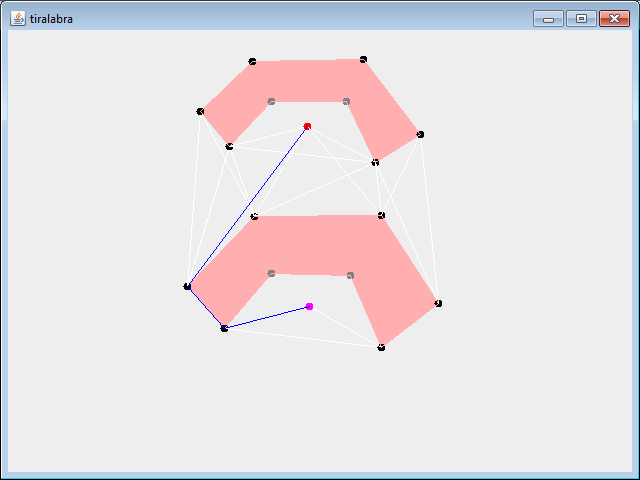
\includegraphics[scale=0.75]{example01.png}} \hspace*{\fill} \\
\centerline{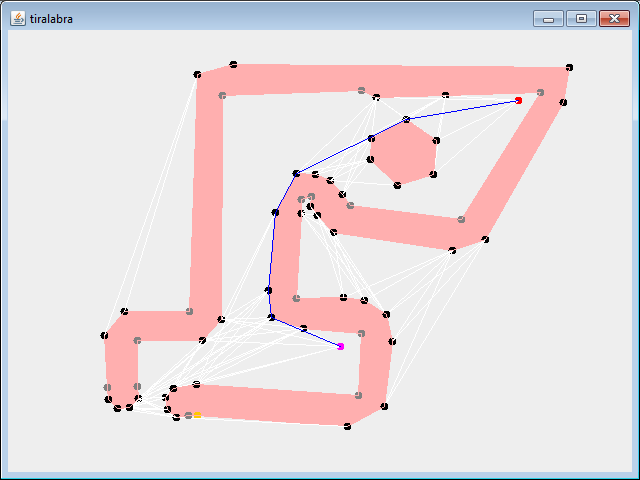
\includegraphics[scale=0.75]{example02.png}} \hspace*{\fill} \\
\centerline{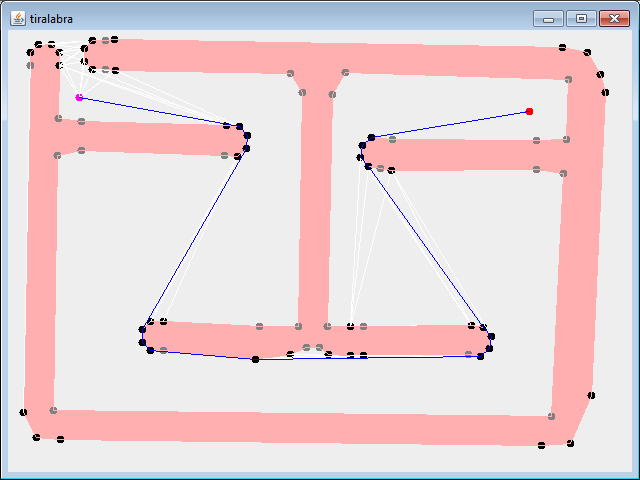
\includegraphics[scale=0.75]{example03.png}} \hspace*{\fill} \\
\centerline{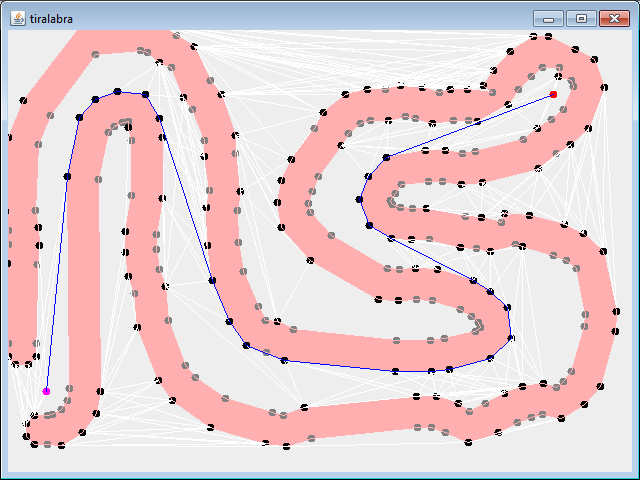
\includegraphics[scale=0.75]{example04.png}} \hspace*{\fill} \\
\centerline{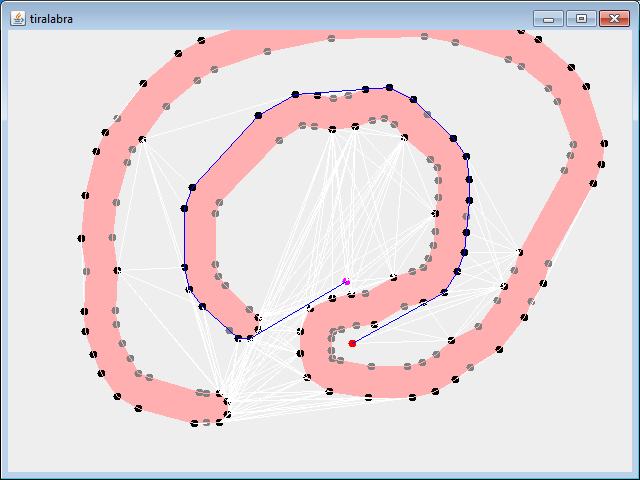
\includegraphics[scale=0.75]{example05.png}} \hspace*{\fill} \\
\centerline{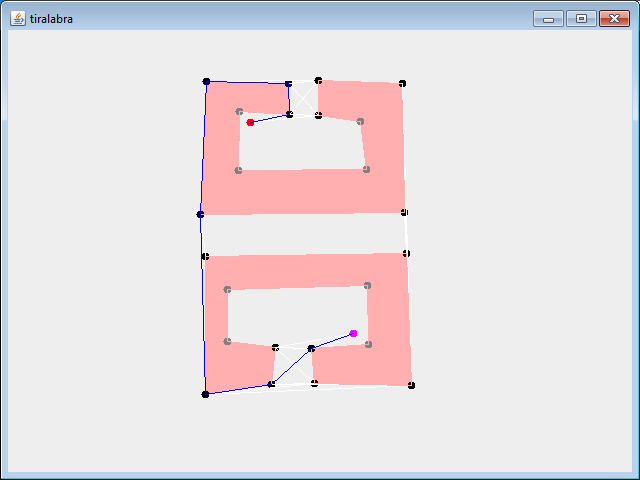
\includegraphics[scale=0.75]{example06.png}} \hspace*{\fill} \\
\centerline{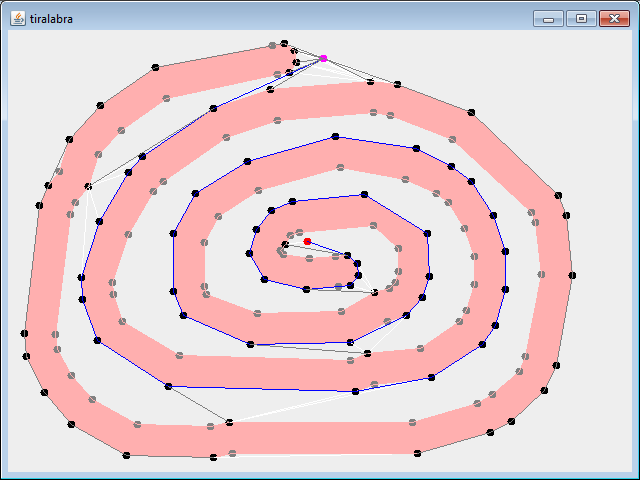
\includegraphics[scale=0.75]{example07.png}} \hspace*{\fill} \\
Next screenshots visualize the A* algorithm, where not all edges in the graph are processed while finding the shortest path. Processed edges are colored gray.\\
\centerline{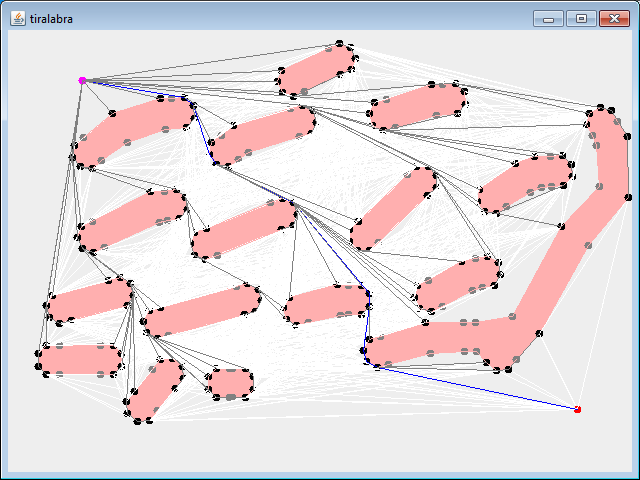
\includegraphics[scale=0.75]{example08.png}} \hspace*{\fill} \\
\centerline{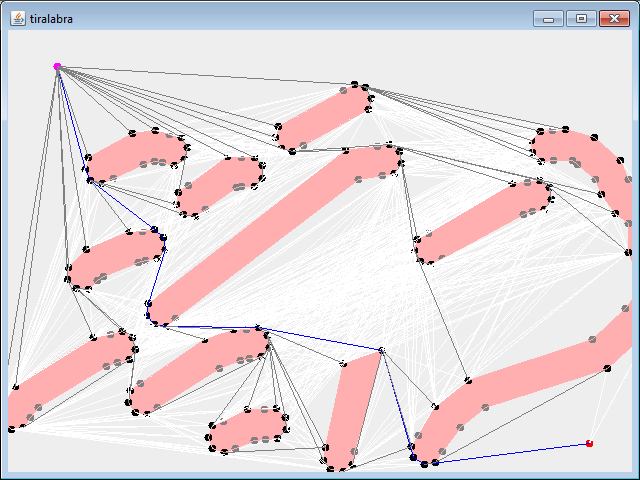
\includegraphics[scale=0.75]{example09.png}} \hspace*{\fill} \\

\end{document}